\paragraph{}
En esta sección entraremos más en detalle en lo que a las mecánicas de
\juego se refiere. Se comentarán todos los pilares que fundamentan su
jugabilidad y se detallarán las acciones que podrá llevar a cabo el jugador
dentro de una partida típica. Además, se ofrecerá una lista con los personajes
del juego (tanto protagonista como enemigos), habilidades, objetos etc.
Por último, se modelará el mundo en el plano de movimiento, físicas y
detección de colisiones.


\subsection{Jugabilidad}
\label{sec:mec-jugabilidad}

\paragraph{Niveles}
Cada nivel de \juego es un piso de la torre sagrada (en orden ascendente)
que nuestro joven mago debe defender. Escenarios interiores
reducidos con varias entradas y un objeto valioso (reliquia) en el centro.
Los invasores acceden al nivel por las puertas y debemos impedir que alcancen
el objeto. Los niveles tendrán obstáculos, sobre todo mobiliario,
que dificultará o el tránsito por algunas zonas. Habremos vencido cuando
las oleadas de enemigos (previamente establecidas) hayan cesado.

\paragraph{Varios focos}
Nuestro personaje se verá sobrepasado por la entrada simultánea de enemigos
en el nivel. La posibilidad de moverse con libertad por las zonas libres
del escenario le permitirá atender los puntos de entrada según el criterio
del \jugador. El movimiento de los personajes será sobre un plano (el suelo)
aunque más adelante se darán más detalles sobre el movimiento.

\paragraph{Intensidad}
La dificultad de \juego viene dada por la cantidad de enemigos asaltando
el nivel, su fortaleza y la distancia entre los distintos puntos de acceso.
Entre niveles la intensidad y dificultad de las partidas irá aumentando en
consonancia al gráfico que se muestra a continuación.

\begin{figure}[H]
    \centering
        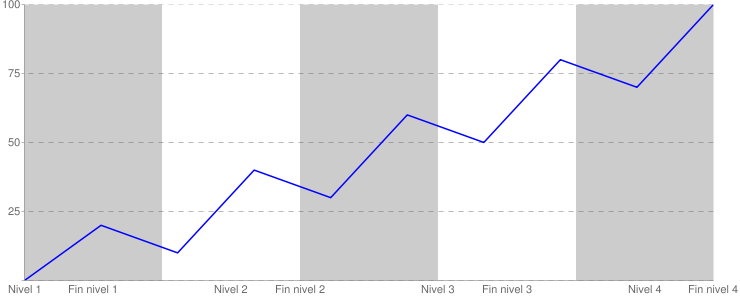
\includegraphics[width=12cm]{img/intensidad.png} 
    \caption{Intensidad de juego a lo largo de los niveles}
    \label{img:intensidad}
\end{figure}

\paragraph{Trampas}
Las trampas conforman una de las herramientas del \jugador para hacer frente
a la invasión. Consumen parte de los recursos del protagonista y pueden
ser útiles para impedir el avance del enemigo o para infligirle daño
si se éste se topa con una. Son elementos estáticos que coloca manualmente
el \jugador.

\paragraph{Habilidades}
Las habilidades inciden en el componente de acción de \juego de forma que
se aleja del clásico Tower Defense. El protagonista debe acudir al foco de
acción que considere oportuno para utilizar hechizos directos que dañarán
a sus enemigos. Existirán varios tipos de habilidades y hechizos cuya efectividad
dependerá de las características del enemigo.

\paragraph{Recursos limitados}
El \jugador no podrá dedicarse a lanzar hechizos y colocar trampas sin
llevar una táctica concreta. El protagonista cuenta con un potencial limitado
(no olvidemos que es un simple iniciado) y debe administrarlo racionalmente.
El protagonista sólo podrá utilizar una habilidad concreta si sus puntos de
\emph{Energía mágica} superan al coste de dicha habilidad. Como veremos en secciones
posteriores, ciertas trampas y habilidades funcionan mejor que otras según
el enemigo y el escenario. Por ejemplo: un hechizo de hielo será mucho más
efectivo contra una criatura débil ante ese elemento que contra otra que lo resista.
Además, un obstáculo de reducido tamaño sólo funcionará si se coloca en un
pasillo de tamaño reducido. El componente táctico es primordial y cobrará mucha
importancia en el desarrollo de una partida.

\paragraph{Progresión del jugador}
El \jugador progresará a medida que avanza por los niveles consiguiendo
nuevas habilidades. De esta forma el \jugador no sólo se verá recompensado
por completar niveles sino por el hecho de que su personaje sea más poderoso.

\paragraph{Planificación de la batalla}
El \jugador tendrá a su disposición un conjunto más o menos amplio de habilidades,
según estas se hayan desbloqueado o no. No obstante, las pobres habilidades
del protagonista le impiden utilizarlas todas al mismo tiempo. Antes de cada
nivel, el \jugador deberá elegir únicamente 5. Con esta decisión se pretende
aumentar el componente táctico de \juego. Por supuesto, de cara al siguiente
nivel, el \jugador podrá volver a elegir el subconjunto de habilidades
que considere oportuno.

\subsection{Flujo de juego}
\label{sec:mec-flujo}

\paragraph{}
A lo largo de esta sección se detallará el transcurso de una partida típica
a \juego. Se comentarán los pasos que ha de seguir el \jugador desde el arranque
del juego hasta completar un nivel completo. Poco a poco vamos desgranando
el funcionamiento exacto del juego, en esta sección describimos las mecánicas.
Más adelante se definirá el contenido de cada pantalla.

\paragraph{}
El \jugador inicia \juego y se le presenta el \menu. Si desea iniciar una
partida el \jugador seleccionará la opción \emph{Jugar}. \juego soporta
varias partidas guardadas en forma de perfiles. En la
siguiente pantalla el \jugador seleccionará el perfil que desee. Si no
cuenta con un perfil creado podrá crear uno nuevo. Entonces,
el \jugador podrá elegir cualquiera de los niveles que haya desbloqueado
en la pantalla de \selnivel.

\paragraph{}
Los niveles se organizan de forma secuencial y cada vez que se completa
uno, se desbloquea el siguiente. Luego, hay que seleccionar el conjunto
de habilidades y trampas de las que dispondrá el protagonista en el transcurso
del nivel (\selhabilidad). El \jugador podrá seleccionar 5 de ellas llenando los slots
(casillas) disponibles

% Desarrollo de una partida
\paragraph{}
El personaje comienza el nivel en el centro del piso y se le advertirá al
\jugador que las oleadas están próximas. Deberá proteger una zona que albergará
alguna reliquia mágica. El \jugador será derrotado si las bestias la alcanzan
o si acaban con la vida del protagonista. Poco a poco aparecerán enemigos
por las entradas del nivel. El \jugador podrá seleccionar en cualquier
momento una de las habilidades o trampas disponibles. Sólo
podrá utilizarlas si su nivel de energía se lo permite. La energía mágica
se irá recargando con el paso del tiempo. Si hemos seleccionado una habilidad,
al pulsar el botón de ataque, ésta será proyectada en la dirección actual.
En cambio, si tenemos una trampa seleccionada, la colocaremos en la posición
deseada. Cuando abatimos a un enemigo recibiremos puntos que nos ayudarán
a desbloquear más habilidades.

\paragraph{}
Si el personaje muere o los enemigos alcanzan la zona que debemos proteger
se mostrará un mensaje de \emph{`Game Over'} y el nivel se reiniciará. No
hay un número determinado de vidas, el \jugador puede repetir un escenario
cuantas veces necesite.

% Fin del nivel
\paragraph{}
Cuando hemos acabado con las oleadas de enemigos del nivel actual
aparece un cartel de \emph{`Victoria'} indicándole al \jugador
que ha completado el piso. Tras la pantalla de \nivel vamos a la de \finnivel.
En ella se nos comunica el progreso que hemos realizado y si hemos
conseguido desbloquear una nueva habilidad. En tal caso, dicha habilidad
aparecerá disponible la próxima vez que acudamos a la pantalla de \selhabilidad.
En el momento en el que el \jugador acepte volveremos a la pantalla de \selnivel con un nuevo
nivel disponible.

\paragraph{}
Cuando lo desee, el \jugador podrá regresar a pantallas anteriores o al
\menu. Más adelante se mostrarán todas la posibilidades de flujo
entre pantallas.

\subsection{Personajes}
\label{sec:mec-personajes}

\paragraph{}
En esta sección procederemos a enumerar y describir todos los personajes
de \juego así como sus habilidades y comportamiento. 

\paragraph{}
Existen habilidades y enemigos afines a algún elemento. Tenemos tres elementos
que se sitúan en forma de triángulo. De esta forma uno es efectivo contra
un segundo pero débil ante un tercero. Dicho triángulo se expone en el siguiente
gráfico:

\begin{figure}[H]
    \centering
        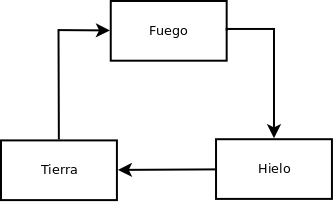
\includegraphics[width=5cm]{img/elementos.png} 
    \caption{Elementos del juego y su relación}
    \label{img:elementos}
\end{figure}

\subsubsection{Protagonista}

% Descripción
\paragraph{Descripción}
\personaje es el protagonista de \juego. Es un iniciado en la torre de los
magos y su misión es protegerla mientras sus compañeros acuden a un rito sagrado.
\personaje es joven, simpático y tiene un carácter apasionado, propio de un
iniciado. Su apariencia es muy sencilla, no lleva ropas de lujo ni adornos dado
su status en la jerarquía de la comunidad mágica. Va armado con un báculo
de iniciado.

% Concept art

\begin{itemize}
    \item \textbf{Vida inicial}: 100 (se restaura en cada nivel)
    \item \textbf{Magia inicial}: 100 (se restaura en cada nivel)
    \item \textbf{Experiencia inicial}: 0
    \item \textbf{Velocidad}: 20
\end{itemize}

% Habilidades
\paragraph{Habilidades}
La siguiente tabla muestra la lista de habilidades de \personaje junto
con una descripción, su coste en energía mágica y la experiencia necesaria
para desbloquearlas.

\begin{table}[H]
    \centering
        \begin{tabular}{| p{2.6cm} | p{7cm} | p{2cm} | p{2cm} | p{2cm} |}
            \hline
            \textbf{Habilidad} & \textbf{Descripción} & \textbf{Daño} & \textbf{Magia} & \textbf{Experiencia}\\
            \hline
            Bola de fuego & Hechizo a distancia del elemento \emph{fuego} & 30 & 20 & 0  \\
			\hline
            Furia de Gea & Ataque a distancia del elemento \emph{tierra} & 30 & 20 & 0  \\
			\hline
            Ventisca & Hechizo a distancia del elemento \emph{hielo} & 30 & 20 & 500  \\
			\hline
        \end{tabular}
    \caption{Hechizos del protagonista}
    \label{tab:hechizos}
\end{table}

% Trampas
\paragraph{Trampas}
La siguiente tabla muestra la lista de trampas de \personaje junto
con una descripción, su coste en energía mágica y la experiencia necesaria
para desbloquearlas.

\begin{table}[H]
    \centering
        \begin{tabular}{| p{2.7cm} | p{7cm} | p{2cm} | p{2cm} | p{2cm} |}
            \hline
            \textbf{Trampa} & \textbf{Descripción} & \textbf{Daño} & \textbf{Magia} & \textbf{Experiencia}\\
            \hline
            Panel de pinchos & Crea un panel en el suelo por tiempo limitado con peligrosos pinchos & 10 & 40 & 0  \\
			\hline
            Muro mágico & Crea un muro semitransparente que impide temporalmente el paso de enemigos & - & 40 & 800  \\
			\hline
            Señuelo & Crea un espejismo de la reliquia del nivel lo que provoca que los enemigos se despisten temporalmente & - & 70 & 1000  \\
			\hline
        \end{tabular}
    \caption{Trampas del protagonista}
    \label{tab:trampas}
\end{table}

\subsubsection{Goblin}

% Descripción
\paragraph{Descripción}
Enemigo básico sin ninguna afinidad elemental. Clásica criatura verde, desagradable
y de baja estatura. Va armado con una tosca espada corta y un burdo taparrabos.
Acuden en gran número (su gran ventaja), son ágiles pero no tienen grandes
habilidades en combate.

\begin{itemize}
    \item \textbf{Vida}: 60
    \item \textbf{Ataque}: 15
    \item \textbf{Velocidad}: 20
    \item \textbf{Afinidad elemental}: ninguna
\end{itemize}

\subsubsection{Diablillo}

% Descripción
\paragraph{Descripción}
Criatura del averno de estatura ligeramente superior al Goblin. Cuenta con
la cola y los cuernos clásicos de los demonios. No lleva ropa y su rojo
oscuro de piel le confiere un aspecto más despiadado. Ataca con sus afiladas
garras y no necesita ningún tipo de arma adicional.

\begin{itemize}
    \item \textbf{Vida}: 70
    \item \textbf{Ataque}: 25
    \item \textbf{Velocidad}: 20
    \item \textbf{Afinidad elemental}: fuego
\end{itemize}

\subsubsection{Gólem de hielo}

% Descripción
\paragraph{Descripción}
Una criatura de gran tamaño formada por bloques de hielo. Su avance es lento
y pesado pero sus golpes son temibles.

\begin{itemize}
    \item \textbf{Vida}: 100
    \item \textbf{Ataque}: 40
    \item \textbf{Velocidad}: 10
    \item \textbf{Afinidad elemental}: hielo
\end{itemize}

\subsubsection{Araña del bosque}

% Descripción
\paragraph{Descripción}
Araña gigante (de menor tamaño que el Gólem) proveniente de un bosque oscuro.
Su armazón le protege de los ataques, sobre todo si éstos son de fuego.

\begin{itemize}
    \item \textbf{Vida}: 80
    \item \textbf{Ataque}: 20
    \item \textbf{Velocidad}: 20
    \item \textbf{Afinidad elemental}: tierra
\end{itemize}

\subsection{Movimiento y físicas}
\label{sec:mec-movimiento}

\subsubsection{Interacción entre elementos}

\paragraph{}
\juego se desarrolla sobre un plano y tanto los enemigos como el personaje
pueden desplazarse por él. De todos modos, el escenario presentará ciertos
obstáculos como paredes o mobiliario que no podrán ser atravesados por
ninguna entidad.

\paragraph{}
Los enemigos atacan cuerpo a cuerpo por lo que han de estar próximos al protagonista
para golpearle. Cuando el \jugador selecciona un hechizo y el objetivo, el 
personaje se girará hacia dicho objetivo y lanzará el proyectil. En cambio,
si el \jugador selecciona una trampa, el protagonista se dirigirá hacia la
posición objetivo seleccionada por el \jugador. Cuando los hechizos colisionan
con un personaje, éste sufre daño y el hechizo se desvanece. Si el hechizo
colisiona con 

\paragraph{}
En definitiva, las colisiones que se producirán:

\begin{itemize}
    \item Personaje - Personaje
    \item Personaje - Escenario
    \item Hechizo - Personaje
    \item Hechizo - Escenario
    \item Trampa - Personaje
    \item Trampa - Escenario
\end{itemize}

\subsubsection{Controles}

\begin{itemize}
    \item \emph{Movimiento}: teclas W,A,S,D.
    \item \emph{Seleccionar habilidades}: click izquierdo sobre la interfaz.
    \item \emph{Usar habilidad}: click izquierdo sobre el escenario. Al utilizar
    la habilidad el personaje se girará hacia el objetivo.
\end{itemize}
